\documentclass[letterpaper]{article}
\usepackage{aaai}
\usepackage{times}
\usepackage{helvet}
\usepackage{courier}
\usepackage{graphicx}
\usepackage{listings}
\usepackage{url}

\setlength\fboxsep{6pt}
\setlength\fboxrule{1pt}

\lstset{
  basicstyle=\footnotesize,
  captionpos=b,
  breaklines=true,
  breakatwhitespace=false,
  frame=single,
  linewidth=83mm,
  xleftmargin=1.5mm,
}

\pdfinfo{/Title (Hybrid Browser / Server Collection of Streaming Social Media Data for Scalable Real-Time Analysis)
/Subject (AAAI Publications)
/Author (AAAI Press)}
\setcounter{secnumdepth}{0}
\begin{document}

\title{Hybrid Browser / Server Collection of Streaming Social\\
Media Data for Scalable Real-Time Analysis}

\author{
Lance Reagan Vick\\
Tawlk\\
4545 36th St.\\
Orlando FL 32807. USA\\
lance@tawlk.com
\And
Titus Soporan\\
Tawlk\\
4545 36th St.\\
Orlando, FL 32807, USA\\
titus@tawlk.com
\And
Daniel Robert Lewis\\
Levelset Labs\\
4442 Sandhurst Dr\\
Orlando, FL 32817, USA \\
daniel@levelsetlabs.com\\
\And
Jane Brooks Zurn\\
School of Engineering \\
Virginia Commonwealth University \\ 
Richmond, VA 23284, USA \\
jbzurn@gmail.com
}
\maketitle

\begin{abstract}
\begin{quote}
We present a novel approach to collecting and distributing social media data in web service projects using both clients and servers for real-time analysis, ultimately providing an inexpensive and scalable method of a quality that has not been available to date. Current challenges to social data mining include vendor enforced API limits and infrastructure costs. Our hybrid client / server approach allows data to be collected via JavaScript in browsers as well as by servers. This allows applications to compute a wide range of data analytics. We present pure client and server based collection strategies, then demonstrate how our method has substantial advantages over both. Specific advantages include lower infrastructure requirements and greater efficieny in API utilization. Our approach distributes the majority of data collection tasks to client web browsers while using servers to supply more complex analysis techniques. In addition, we provide details on two open source tools we have released to facilitate implementation by researchers in their own projects. We close by detailing a use case scenario describing a large scale public web service project followed by a solution accomplished using our approach and open source tools.
\end{quote}
\end{abstract}

\section{Introduction}

Social media data is an emerging and increasingly valuable resource.  It has been shown relevant for diverse topics including consumer confidence and political opinion \cite{tweetspolls,germantwitter}, and gauging sentiment on a societal scale \cite{10.1371/journal.pone.0026752}.    Groups using these tools range from retail chains \cite{target} to the United Nations\footnote{\url{http://www.unglobalpulse.org/}}. In addition, the stream of social media data has a cyclical nature depending on time of day and year \cite{facebookrhythms}, and current events may appear in the stream before they are reported by traditional media venues \footnote{\url{http://mashable.com/2012/02/12/whitney-houston-twitter/}}.

One of the most sought-after goals in the industry of social media data mining and analysis is development of web services that can collect, normalize, and analyze unstructured data in real-time. This goal is now especially feasible for many projects. Many major social media services, such as Facebook and Twitter, have released APIs that allow the collection of user generated data from their services at no cost. Once one has a reliable mechanism in place to collect and distribute this information, a nearly endless variety of data analysis and user engagement applications become possible.

With many of today's tools it is possible to collect social media data in a way that scales well to the general public, with low infrastructure expense \cite{miningsocialweb}. In spite of vendor-enforced limitations, like API limits, strategies exist for reliably mining large amounts of data from social media sources. It is common to acquire social data using centralized servers \cite{5992588}. In this paper, we refer to this method as the ``Server Collection'' approach. This is ideal in some situations, but a large number of servers can prove too costly for many project budgets. Another possible way to collect and analyze large quantities of this data is by using independent client browsers (here called the ``Browser Collection'' approach). Each browser, however, is limited to the data it can acquire on its own and the analysis capabilties it can offer. This limits the possibilities for large scale analytics.

We present a novel approach, ``Hybrid Collection Model (HCM)'', for reliably collecting and distributing volumes of social media data in a way that reduces infrastructure costs and avoids violating API limits. The HCM is a strategy for dividing API calls and computation tasks as appropriate between both client browsers and servers. This approach makes it possible to gain knowledge from a diverse range of real-time social network data feeds without the need to gather all data using a large number of centralized servers. The HCM can be implemented with a combination of a variety of open-source tools, including some released by members of our team. These allow scalable data acquisition, processing, and analysis for web services. Researchers can modify the recommended open-source components or choose their own. Thus, the model is library and language agnostic, enhancing its flexibility so that users can improve performance without the expense of building a complete system from scratch.

\section{Background}

This section provides details on the problem of real-time data collection and the acquisition approaches that contribute to our method.

\subsection{API Limitations}

Currently, most major public social networks vital for inclusive social media data research endeavors enforce fairly strict throttles and limitations on requests. At the time of this writing the following limitations exist:

\subsubsection{Twitter} 
\begin{itemize}
\item maximum of 400 track keywords
\item maximum of 5000 follow userids
\item maximum of 1\% of total public data stream
\end{itemize}
At the time of this writing elevated access to 50\% of the complete real-time Twitter API runs approximately \$360,000.00 USD per year from their partner provider Gnip.

\subsubsection{Facebook} 
\begin{itemize}
\item maximum of 600 per 600 seconds per token and per IP
\item maximum of 50 operations in one batch request
\end{itemize}
At the time of this writing Facebook has made no public process available to appeal for higher access.

\subsubsection{Google+}
\begin{itemize}
\item maximum of 5 requests per second
\item maximum of 1000 queries per day per API key
\end{itemize}
Google provides an application process to appeal for higher access. Our experience was that elevated access was granted after approximately three months.

\subsubsection{Other Services}

Other APIs, such as Reddit, Delicious, and Digg, may not specify limits but will often temporarily, and in some cases permanantly, deny access after a significant amount of use in a limited period of time.

\subsection{Server Collection}

Dividing data collection tasks across multiple systems, each with their own unique network identities, is one approach for getting needed data while still respecting API limits. In most instances these limits are enforced on a per-IP basis thus an increased number of servers with unique IP addresses can still allow larger amounts of data to be collected.

Though effective in many situations, this strategy comes at a cost of high resource needs. The number of unique IP addresses and servers required to track increases steadily as needs for more unique keywords to track arise. In order to potentially reduce API calls, and by extension the number of servers required, a dedicated data storage or caching strategy is also often needed. This strategy also requires that layers of infrastructure exist between the browser and collected data. A scalable bidirectional communications strategy utilizing Comet methods or WebSockets, and supporting infrastructure, is often required to keep updates streaming to users in real-time.

%An in-memory key/value system like Redis or an AMQP solution like RabbitMQ will often be required to adequately and reliably stream real-time data to a large number of clients. These details alone indicate this strategy can be very demanding on resources, and thus can be very costly to support for scaling to a large number of clients. Also it may occur that a large number of clients suddenly connect to your web service demanding more social network API connections or processing operations than the present state of your infrastructure can support. When this happens, some clients may have to wait to receive data a significant amount of time for a server to become available, for a new server to be deployed, or for an avaliable quota in respect to API limits.

\subsection{Browser Collection}

To avoid placing the full weight of data collection on limited back-end server resources, JavaScript code running in the client browsers can be used instead. This allows collection tasks to be distributed across all clients accessing a web service. This is possible because most major social media API providers implement JSON-P which takes sets of JSON data and masquerades it as a JavaScript file, thus bypassing the Same Origin Policy enforced by all major browser vendors. Because every client browser gets its own set of API limits, all requests are bound to a web services users rather than to one of its servers. This results in minimal back-end servers being required.

Though an ideal solution for some projects, this method currently has some disadvantages. Important data points are not available via browser-acessible API methods like JSON-P without providing a server configured to act as a proxy. In particular, at the time of this writing Twitter does not include the number of followers for a given user in their public search API, which can be critical for some data analysis tasks. Also, due to the Same Origin Policy, browser vendors force projects to be limited to services that offer API methods that bypass the Same Origin Policy, like JSON-P. This means that many other potential feed resources such as RSS or ATOM are unable to be directly used in the Browser Collection strategy. Also, the exclusive reliance on only client-side JavaScript results in all data analysis methods being open-source by design, which is undesirable or legally impossible in some circumstances.

\section{Methodology}
A hybrid of the above Browser Collection and Server Collection strategies can share many of the advantages, and eliminate many of the disadvantages, of both approaches. To our knowledge this method has not been presented by another group. This section describes the implementation of a Hybrid Collection Model (HCM).

\subsection{Hybrid Collection Model}
The Hybrid Collection Model (HCM) is a strategy for acquiring and processing social media data intended to have minimal infrastructure requirements while also minimizing API feed usage from any single machine. The approach is modular, which increases flexibility and ease of scaling for a wide range of projects, without large structural changes. Bulk data can be collected in real-time by client browsers using a client-side JavaScript library specialized for this purpose. The browser-collected data can be sent to the server for analysis via any number of bi-directional protocols (such as Websockets) and echoed back to the browser once analyzed, providing real-time analysis as new data is made available. Supplemental data that requires more processing and collection time can be done in batches on the server side, without affecting the results streaming to the browser. Data points missing in JSON feeds can be supplemented by the server feeds. Statistics can be buffered and supplied pre-rendered to client browsers when available. The local JavaScript collection can use these statistics as a starting point and refine these statistics remotely for real-time results. Server requirements are limited to what is needed to meet redundancy and/or passive data analysis requirements. In many situations, the server requirements (and by extension, the recurring costs) of the complete data mining platform are vastly reduced.

\begin{figure}[h!]
    \fbox{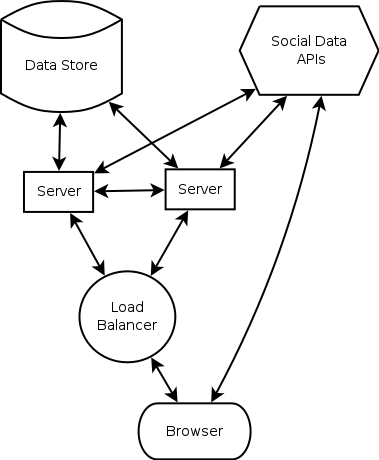
\includegraphics[width=79mm]{figures/figure3.png}}
    \caption{Hybrid Browser/Server Collection Model}
\end{figure}

While flexibility is greatly increased, caution must be used in how collected data is handled in respect to data poisoning possibilities. Data poisoning occurs when a malicious user sends the server falsified data for analysis. One approach for avoiding this is to analyze and echo data points only back to the users that request them. There is also a possibilty for accountability systems to catch most if not all falsified data. This is left for future research.

\section{Tools}

In order to make the HCM model work, both client side and server side data collection modules are required, capable of sharing the same basic data formats. To this end, we developed tools to fulfill each of these roles, and have provided both libraries as free open source software under an AGPLv3 license. Both tools also share a normalized data format called USMF making it ideal for storage, analysis, and transporting back and forth between both systems.

\subsection{Hyve}

Hyve\footnote{\url{http://github.com/tawlk/hyve}} is a framework agnostic JavaScript library that, at the time of this writing, can continuously poll a range of social networks and retrieve any public social media activities made available by their API's that match given query terms. Many networks are supported, such as Facebook, Twitter, and Youtube. The library was designed with measures to provide stability and reduce API calls by caching methods such as HTML5 localStorage. Special considerations are also made to reduce browser memory and cpu usage, for instance, continually cleaning unneeded DOM references as data is collected, and network-specific optimizations such as only polling Twitter for items newer than the most recent item collected. The library is modular and can be easily extended to provide support for networks not included in the core library.

Applications include any web-based system which requires access to live streaming social media data from any given query.  This streaming data can be directly passed off to other JavaScript code or the server for rendering or analysis in real time, via a callback function.

\subsection{Kral}

Kral\footnote{\url{http://github.com/tawlk/kral}} is a Python library designed to stream data from major public social media channels that match given queries. It is event driven using the Eventlet library which allows it to have many asynchronous operations occurring at once while still maintaining a relatively low memory footprint. Kral respects API limits and can utilize static JSON feeds like those provided by Facebook or streaming APIs such as that provided by Twitter. These are all available to be integrated into existing code as a Python generator. Kral, like Hyve, is designed to be modular and easy to extend with new networks.

Kral is ideal for continuously collecting real-time data for storage and statistical analysis over a long period of time. It can be used to suppliment data points that cannot be collected by front-end solutions like Hyve, such as Twitter follower counts.

\section{Use Case Scenario}

In order to demonstrate how the HCM approach can be particularly useful in production, consider the following use case:

A project is in planning stages and has a specific set of criteria. The project goal is to grant a user from the general public the ability to enter a query and receive a real-time streaming feed of social media results related to that query. The results also must be provided alongside a series of periodically updated statistics, such as averages of \textit{Popularity} based on posts per second, \textit{Sentiment} based on the negative or positive sentiment for each post, and \textit{Amplification} based on the average number of users who subscribe to each posts' author.  Additionally, the project budget is only large enough to offset the cost of two dedicated servers each with its own IP address.

\section{Solution}

One might try to solve this problem with either the Browser Collection or Server Collection strategies. It would quickly be discovered that the Browser Collection strategy will be unable to provide an Amplification statistic, as Twitter does not provide follower counts via their JSON-P search API. The Server Collection strategy would also fail as API limits would prevent real time collecton for a large number of clients requesting different queries. This would fail because of the availability of only two IP addresses to distribute the requests over.

One possible solution to this problem would be to implement the HCM using Hyve for the browser-side collection portion and Kral for server-side collection. A machine learning-driven sentiment analysis engine could be installed on the servers to generate classifiers. Custom Amplification analysis code can also reside on the servers to provide periodically updated Amplification calculations.

In this solution, the process begins with an end user entering a query into the public web interface. This triggers Hyve, which is loaded into the browser, to immediately start polling social media APIs client-side. Simultanously, a bidirectional HTTP framework, like SockJS, initiates the connection and begins to route browser-collected data to and from the servers. A load balancer proxy service, such as HAProxy, intelligently routes SockJS and HTTP connections over the same network port.

\section{Results}

This strategy outlined in the Solution section allows the majority of the application to function in real-time, with minimal processing. The requirement of only two servers as outlined in the Use Case Scenario section is also fufilled. This is possible because the servers are tasked only with periodically updating the one missing Amplification statistic, calculating sentiment in memory, and serving the interface. Interface serving load is also mitigated by using HTML5 Offline Storage to further conserve overall infrastructure resources.

In practice we have had great success with this strategy. We have successfully deployed a public production web service designed to meet very similar requirements to those outlined in the Use Case Scenario. Our service utilizes a heavily customized combination of Tornado, SockJS-Tornado, SockJS-Client, Redis, Synt, Hyve, Kral, and proprietary analysis methods. This service can be observed publically via http://tawlk.com. In several months of monitoring this iteration of our service, we have seen only marginal system resource utilization on two modest servers. This has remained true even under a load of hundreds of simultaneous clients collecting and analyzing social media data in real-time.

\section{Conclusion}

In this paper, we presented the Hybrid Collection Model (HCM), a novel hybrid browser / server collection approach to harvesting social media data for real-time analysis in an inexpensive and scalable way. Several open-source tools proved useful for this flexible and modular framework. Some key tools examined include Hyve and Kral. We demonstrated operation of HCM by describing a Use Case Scenario involving acquisition of real-time data from social media APIs and statistical calculations provided as a public web service. HCM was more effective and efficient at performing this task than other presented strategies, including Browser Collection and Server Collection. 

\section{Future work}

We are currently researching Naive Bayes classifiers capable of running in a browser to further reduce server reliance in data projects. We will also explore accountability systems for browser collected data to make it more suitable for aggregated storage and semi-supervised classification systems. Another goal is promotion of a standardized format for all projects that utilize social media data. Currently we are focusing our efforts on developing the USMF format used in Hyve and Kral. Future research will also include examination of correlations found in time-series social media data to other media such as stock prices and public poll data.

\section{Acknowledgements}

We would like to thank Burton J. Grippin, Spencer C. Judd, Andrew Miller, David T. Pflug, Stuart B. Powers, William L. Starkweather, Jamie A. D. Szafran, and Steven J. VanHorn, for their respective efforts in providing helpful commentary and critique to this paper during the authoring process.

\bibliography{references}

\bibliographystyle{aaai}

\end{document}
​